\section{Auswertung} \label{sec:Auswertung}
Die zur Verfügung gestellten Messdaten sind im Folgenden tabellarisch aufgelistet:

\begin{table}[H]
\centering
\caption{Aufgenommene Messdaten.}
\label{tab:Messdaten}
\sisetup{table-format=2.1}
\begin{tabular}{c c c c c c}
\toprule
$t \mathbin{/} \si{\minute}$ &
$T_1 \mathbin{/} \si{\celsius}$ &
$p_1 \mathbin{/} \si{\bar}$ &
$T_2 \mathbin{/} \si{\celsius}$ &
$p_2 \mathbin{/} \si{\bar}$ &
$N \mathbin{/} \si{\watt}$ \\
\midrule
\expandableinput{build/table_messdaten.tex}
\bottomrule
\end{tabular}
\end{table}

\newpage
\subsection{Diagramm der gemessenen Temperaturverläufe} % a)
In \autoref{fig:plot} sind die Approximationen aus \autoref{eqn:approx_poly} in \autoref{sec:approx} bereits enthalten.
Dargestellt sind die zeitlichen Verläufe der Temperaturen $T_1$ und $T_2$.

\begin{figure}
  \centering
  \includegraphics{build/wärmepumpe_plot.pdf}
  \caption{Temperaturverläufe in Abhängigkeit der Zeit $t$.}
  \label{fig:plot}
\end{figure}

\subsection{Approximation der Temperaturverläufe} \label{sec:approx} % b)
Zur Approximation des Temperaturverläufe bietet sich ein Polynom zweiten Grades an:
\begin{equation}
  \label{eqn:approx_poly}
  T(t) = At^2 + Bt + C \; .
\end{equation}

Als Fit-Parameter wurden berechnet:

\begin{table}[H]
\centering
\caption{Fit-Parameter.}
\label{tab:fit_params}
% \sisetup{table-format=2.1}
\begin{tabular}{c c c c}
\toprule
&
$A \mathbin{/} \si{\kelvin\per\square\second}$ &
$B \mathbin{/} \si{\kelvin\per\second}$ &
$C \mathbin{/} \si{\kelvin}$ \\
\midrule
\expandableinput{build/table_polyfit.tex}
\bottomrule
\end{tabular}
\end{table}

\subsection{Berechnung von Differentialquotienten} % c)
Mithilfe der Approximation aus Gleichung \autoref{eqn:approx_poly} werden nun für vier verschiedene Temperaturen konkrete Differentialquotienten $\frac{\mathrm{d}T_1}{\mathrm{d}t}$ und $\frac{\mathrm{d}T_2}{\mathrm{d}t}$ berechnet.
Die Ableitung des Polynoms lautet:
\[
\frac{\mathrm{d}T}{\mathrm{d}t} = 2At + B \; .
\]
\\

Fehlerrechnung:
\begin{align*}
  \symup{\Delta} \frac{\mathrm{d}T}{\mathrm{d}t}
  &= \sqrt{\left(\frac{\partial \frac{\mathrm{d}T}{\mathrm{d}t}}{\partial A} \cdot \symup{\Delta} A\right)^2 + \left(\frac{\partial \frac{\mathrm{d}T}{\mathrm{d}t}}{\partial B} \cdot \symup{\Delta} B\right)^2} \\
  &= \sqrt{(2t \cdot \symup{\Delta} A)^2 + (\symup{\Delta} B)^2} \; .
\end{align*}

\begin{table}
\centering
\caption{Ableitungen der Approximationsfunktion.}
\label{tab:derivatives}
\sisetup{table-format=2.1}
\begin{tabular}{c c c}
\toprule
$t \mathbin{/} \si{\minute}$ &
$\frac{\mathrm{d}T_1}{\mathrm{d}t} \mathbin{/} \si{\kelvin\per\minute}$ &
$\frac{\mathrm{d}T_2}{\mathrm{d}t} \mathbin{/} \si{\kelvin\per\minute}$ \\
\midrule
\expandableinput{build/table_ableitungen.tex}
\bottomrule
\end{tabular}
\end{table}


\subsection{Bestimmung der Güteziffern} % d)
\label{sec:auswertung_gueteziffern}
% In "Daten und Hinweise" ist lediglich die Rede vom *Fassungsvermögen*!
% „Fassungsvermögen der Wassereimer: m = 4kg“
% Als Füllmenge nehmen wir daher 4L an, wie es in "Daten.dat" steht

% „Wärmekapazität der Kupferschlangen“ meint *Wärmekapazität jeder Kupferschlange*, oder?
Jeder Wassereimer war mit $\SI{4}{\liter}$ Wasser befüllt.
Die Wärmekapazität der \enquote{Kupferschlangen} war gegeben als $m_k c_k = \SI{750}{\joule\per\kelvin}$.
Laut Versuchsanleitung soll $m_k c_k$ auch die Wärmekapazität der Eimer enthalten,
dazu liegen jedoch keine weiteren Daten vor.
Die Wärmekapazität des Wassers in Reservoir 1 lässt sich mit
\begin{align*}
  \rho_\text{Wasser} &= \SI{0.998207}{\kilo\gram\per\liter}
  \tag*{(Wasserdichte bei $\SI{20}{\celsius}$ \cite{wasserdichte})} \\
  \\
  c_\text{Wasser} &= \SI{4.1851}{\joule\per\gram\and\kelvin}
  \tag*{(spezifische Wärmekapazität bei $\SI{20}{\celsius}$ \cite{wasserwaermekapazitaet})} \\
  \\
  C_{\text{Wasser}, 1} &= m_1 \cdot c_\text{Wasser} \\
  &= (\rho_\text{Wasser} \cdot V_\text{Wasser}) \cdot c_\text{Wasser} \\
  &= \left(\SI{0.998207}{\kilo\gram\per\liter} \cdot \SI{4}{\liter}\right) \cdot \SI{4.1851}{\joule\per\gram\and\kelvin} \\
  &= \SI{16710.38}{\joule\per\kelvin} \\
\end{align*}
bestimmen, sodass aus einfacher Summation die gesamte Wärmekapazität
\[
C_\text{ges} = 750 \si{\joule\per\kelvin} + \SI{16710.38}{\joule\per\kelvin} = \SI{17460.38}{\joule\per\kelvin}
\]
folgt.

\ \\
Unter Zuhilfenahme von \autoref{eqn:reale_gueteziffer} und der Differentialquotienten aus \autoref{tab:derivatives} kann nun die reale Güteziffer für verschiedene $t$ berechnet werden.

\begin{table}
\centering
\caption{Vergleich der idealen und realen Güteziffern.}
% \sisetup{table-format=2.1}
\begin{tabular}{c c c}
\toprule
$t \mathbin{/} \si{\minute}$ &
$\nu_\text{ideal}$ &
$\nu_\text{real}$ \\
% TODO: Abweichung in % dazu?
\midrule
\expandableinput{build/table_gueteziffern.tex}
\bottomrule
\end{tabular}
\end{table}

\subsection{Bestimmung des Massendurchsatzes} % e)

Mithilfe der in \autoref{sec:massendurchsatz} aufgeführten Formeln
lässt sich der Massendurchsatz für verschiedene Zeitpunkte bestimmen.
Als Zwischenschritt wurde die Verdampfungswärme zu $L=\SI{118 \pm 6}{\joule\per\gram}$ berechnet.
(Dieser Wert stimmt mit Literaturwerten in etwa überein. \cite{verdampfungswaerme})
\autoref{fig:massendurchsatz_regression} zeigt die dabei durchgeführte Regression.

\begin{figure}
  \centering
  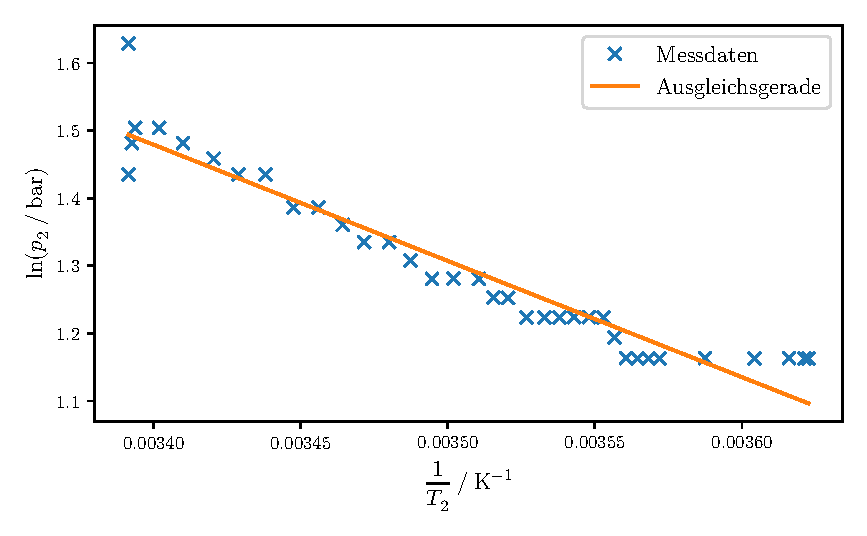
\includegraphics{build/plot_massendurchsatz.pdf}
  \caption{Visualisierung der durchgeführten linearen Regression.}
  \label{fig:massendurchsatz_regression}
\end{figure}

\begin{table}
\centering
\caption{Massendurchsatz.}
% \sisetup{table-format=2.1}
\begin{tabular}{c c c}
\toprule
$t \mathbin{/} \si{\minute}$ &
$\frac{\mathrm{d}T_2}{\mathrm{d}t} \mathbin{/} \si{\kelvin\per\minute}$ &
$\frac{\mathrm{d}m}{\mathrm{d}t} \mathbin{/} \si{\gram\per\second}$ \\
\midrule
\expandableinput{build/table_massendurchsatz.tex}
\bottomrule
\end{tabular}
\end{table}

\FloatBarrier

\subsection{Bestimmung der Kompressorleistung} % f)
Im Folgenden wird die mechanische Leistung des Kompressors berechnet,
die dieser abgibt,
wenn er zwischen den Drücken $p_1$ und $p_2$ arbeitet.

Folgende Daten für $\mathrm{Cl}_2 \mathrm{F}_2 \mathrm{C}$ waren bereits gegeben:
$ρ_0 = \SI{5.51} g/l$ bei $T_0 = \SI{0}{\celsius}$ und $p_0 = \SI{1}{\bar}$, $κ = 1.14$

Durch Umformen der idealen Gasgleichung kann $\rho(t)$ folgendermaßen ausgedrückt werden:
% Ich habe bei der Umformung eine andere Gleichung herausbekommen, aber diese gibt schönere Werte…
\begin{equation*}
  \rho(t) = \frac{p_2(t) \cdot \rho_0 \cdot T_0}{p_0 \cdot T_2(t)} \; .
\end{equation*}

Einsetzen von $\rho(t)$ und den zuvor bestimmten \hyperref[tab:derivatives]{Differentialquotienten} in \autoref{eqn:N_mech} liefert dann Werte für $N_\text{mech}$,
die in der folgenden Tabelle aufgelistet sind.

\begin{table}
\centering
\caption{Kompressorleistung.}
% \sisetup{table-format=2.1}
\begin{tabular}{c c c}
\toprule
$t \mathbin{/} \si{\minute}$ &
$\rho \mathbin{/} \si{\gram\per\liter}$ &
$N_\text{mech} \mathbin{/} \si{\watt}$ \\
\midrule
\expandableinput{build/table_kompressorleistung.tex}
\bottomrule
\end{tabular}
\end{table}
